% !TEX root = ../main.tex

%************************************************
\chapter{Introduction}
\label{ch:intro}
%************************************************

\section{The AGN-Host Galaxy Connection}

Super-massive black holes (BHs) are found at the centres of most nearby massive galaxies and the BH mass and mass of the host galaxy spheroid are strongly correlated \citep{ferrarese00,gebhardt00,kormendy13}. 
Although any underlying causal mechanism(s) responsible for the correlation is yet to be conclusively identified, there is considerable observational and theoretical support for a `feedback' relationship in which the energy output from rapidly accreting BHs - quasars - couples with the gas in the host galaxy and quenches star formation \citep[e.g.][]{king15}. 

Quasar feedback has also been invoked to explain the similarity of black hole accretion and star formation histories.
The number density of quasars, which evolves strongly with redshift, peaks at redshifts $2 \lesssim z \lesssim 3$ \citep[e.g.][]{brandt05,richards06b} and the most massive (M$_{\rm BH} \gtrsim 10^9\msun$) present-day BHs experienced much of their growth during this epoch.  
The star formation rate, which closely follows the cosmological evolution of the quasar luminosity function, also peaks during this epoch \citep[e.g.][]{boyle98}. 
Quantifying the growth-rate of massive BHs at $2 \lesssim z \lesssim 3$ would therefore help significantly in understanding the role quasars play in galaxy evolution.

\section{Measuring Black Hole Masses}

Reliable estimates of BH masses are a prerequisite for investigating the relationship between BHs and their host galaxies.  

\subsection{Reverberation Mapping}

Contiuum variability is a common characteristic of quasars. 
Because the BLR is photoionized by the continuum, the broad emission lines also vary with some characteristic lag, which is related to the light travel time across the BLR. 
The reverberation mapping technique uses the time lag between variations in the continuum emission and correlated variations in the broad line emission to mesaure the typical size of the BLR. 
If we assume that the broad line region dynamic are virialised and the gravitational potential is dominated by the BH, then the BH mass is simply given by the product of the typical BLR radius and the square of the virial velocity of the BLR clouds. 
In practice, reverberation mapping relies on dense spectropotometric monotoring campagins which span many years. 
The typical veloicity in he BLR is measured from the width of he broad \hb lines in the RMS spectra, ensuring that only the variable part of the line contributes to the line width calculation. 
Since the structure and geometry of the BLR is unknown, a virial coefficient $f$ is introduced to transform the observed line-of-sight velocity infered from the line width in to a virial velocity. 
In practice, the value of is empirically determined by requiring that the derived masses are consistent with those predicted from the M-$\sigma$ relation for local inactive galaxies. 
Although this technique has proved to be effective, because it relies on resource-intensive spectro-photometric monitoring campaigns, masses have been derived for only $\sim50$ AGN, all at low redshifts $z\lesssim0.3$. 

If the line-emitting clouds in the broad line region (BLR) are assumed to be virialized and moving in a potential dominated by the central BH, then the BH mass is simply a product of the BLR size and the square of the virial velocity.
The reverberation-mapping technique uses the time lag between variations in the continuum emission and correlated variations in the broad line emission to measure the typical size of the BLR \citep{peterson93,peterson14}. 
The full width at half maximum (FWHM) or dispersion ($\sigma$; derived from the second moment) velocity of the prominent broad emission line of \hb (4862.7\AA)\footnote{Vacuum wavelengths are employed throughout the thesis.} is used as an indicator of the virial velocity, with extensions to other low-ionization emission lines such as \ha (6564.6\AA) and \ion{Mg}{II}\ll2796.4,2803.5 \citep[e.g.][]{vestergaard02,mclure02,wu04,kollmeier06,onken08,wang09,rafiee11}.
Extensive reverberation mapping campaigns have provided accurate BH masses for $\sim$50 active galactic nuclei (AGN) at relatively low redshifts and of modest luminosity \citep[e.g.][]{kaspi00,kaspi07,peterson04,bentz09,denney10}. 

\subsection{Single-Epoch Virial Estimates}

Single-epoch virial BH mass estimates normally take the form

\begin{equation}
  \label{eq:virialmass}
  \mathrm{M_{BH}} = 10^{a} \left( \frac{\Delta V}{1000~\mathrm{km~s^{-1}}} \right)^b \left[ \frac{L_{\lambda}}{10^{44}~\mathrm{erg~s^{-1}}} \right]^c
\end{equation}

\noindent where $\Delta V$ is a measure of the line width (from either the FWHM or dispersion), $L_\lambda$ is the monochromatic continuum luminosity at wavelength $\lambda$, and $a$, $b$, and $c$ are coefficients, determined via calibration against a sample of AGN with reverberation-mapping BH mass estimates. Several calibrations have been derived using different lines (e.g. \hbns, \ion{Mg}{II}, \ion{C}{IV}) and different measures of the line width (FWHM or dispersion) \citep[e.g.][]{vestergaard02,mclure02,vestergaard06,mcgill08,wang09,rafiee11,park13}.

Reverberation mapping campaigns have also revealed a tight relationship between the radius of the BLR and the quasar optical (or ultraviolet) luminosity \citep[the $R-L$ relation; e.g.][]{kaspi00,kaspi07}.
This relation provides a much less expensive method of measuring the BLR radius, and large-scale studies of AGN and quasar demographics have thus become possible through the calibration of single-epoch virial-mass estimators using the reverberation-derived BH masses \citep[e.g.][]{greene05b,vestergaard06,vestergaard09,shen11,shen12,trakhtenbrot12}.
The uncertainties in reverberation mapped BH masses are estimated to be $\sim 0.4$ dex \citep[e.g.][]{peterson10}, and the uncertainties in virial masses are similar \citep[e.g.][]{vestergaard06}.
Since the structure and geometry of the BLR is unknown, a virial coefficient $f$ is introduced to transform the observed line-of-sight velocity inferred from the line width in to a virial velocity.
This simplification accounts for a significant part of the uncertainty in virial BH masses \citep[in addition to, for example, describing the BLR with a single radius $R$ and scatter in the $R-L$ relation;][]{shen13}. 
Furthermore, if the BLR is anisotropic \citep[for example, in a flattened disk; e.g.][]{jarvis06} then the line width will be orientation-dependent \citep[e.g.][]{runnoe13b,shen14,brotherton15}. 

For example, single epoch estimates have been used to calculate black hole masses in the highest redshift quasars to study the growth of SMBHs. 
This figure shows a compilation of SE mass estimates for quasars over a wide redshift range from different studies. These studies show that massive, $10^9$ BHs are probably already in place by $z\sim7$, when the age of the Universe is less than 1 Gyr.
This places strong constraints on BH growth models. 
Single epoch masses have also been used to study the distribution of quasars in the BH mass-luminosity plane, which conveys important information about the accretion process of these active black holes (e.g. Kollmeier et al. 2016). 
Reshift evolution of BH-bulge scaling relations (e.g. Bennert et al. 2011). 
Clustering (Shen \& Ho 2014; Timins et al.?). 

An {\it active galactic nucleus}, or AGN, is an energetic, non-stellar phenomena in the central region of a galaxy. AGN are powered by the accretion of gas, primarily through an accretion disk, onto a central {\it super-massive black hole} (SMBH) of mass $10^{6 - 9}$ M$_\odot$ \citep{lynden-bell69}. With bolometric luminosities in the range $10^{44 - 48}$ ergs$^{-1}$, they are the most luminous persistent sources of radiation in the Universe. 

\section{Orientation-Based Unification Models}

\begin{figure}
  \centering
  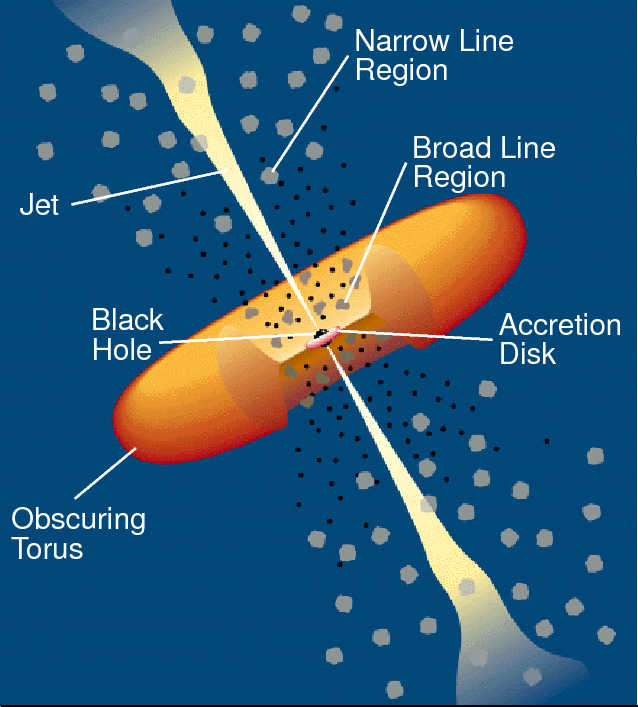
\includegraphics[width=0.5\textwidth]{figures/chapter05/urry_model}
  \caption[{Illustration of the physical structure of an AGN in a simple orientation-based unification model.}]{Illustration of the physical structure of an AGN in a simple orientation-based unification model. Figure taken from \citet{urry95}.}
  \label{fig:agnmodel}
\end{figure}

Unification models attempt to explain all further observational differences as being apparent differences due to {\it orientation} effects. 
The basic physical structure of an AGN in this model is illustrated in Figure \ref{fig:agnmodel}. 
Material is pulled towards the SMBH at the centre and sheds angular momentum through viscous and turbulent processes in an accretion disk, which radiates primarily at ultraviolet (UV) to soft-X-ray wavelengths. 
Strong optical and UV emission lines are produced in photo-ionised gas clouds moving rapidly in close proximity to the SMBH. 
The doppler-broadened emission line widths imply gas cloud velocities of thousands of km s$^{-1}$ in this {\it broad-emission line}. 
Further out are dusty, molecular clouds, the geometry of which is often modelled as a torus co-planar with the accretion disk. 
Along some lines of sight from the observer to the accretion disk / broad line region the dusty torus obscures the UV/optical radiation. 
In this case, an observer would see a weak UV/optical continua and no broad emission lines and classify the AGN as being {\it Type II}. 
On the other hand, if the line of sight is unobscured by the dusty torus then a broad emission line component would be observable in the spectrum and the AGN would be classified as being {\it Type I}. 
Further away from the central black hole and beyond the dusty torus are slower moving clouds of gas which are photo-ionised by the continuum emission from the accretion disk and produce forbidden emission lines of narrower widths (typically hundreds of km s$^{-1}$). 
Outflows of energetic particles occur along the poles of the accretion disk and form collimated radio-emitting jets and in some cases giant radio-emitting lobes. 

While an orientation-based unification scheme such as this is somewhat successful at explaining many of the observational properties of AGNs, other factors such as the host galaxy morphology and gas/dust content may also be important \citep{peterson95}. 
It is also doubtful whether the geometry of the dusty torus is the same in all AGNs, and the fraction of obscured quasars has been shown to decrease with increasing nuclear luminosity \citep{lawrence91}. 
In this scenario of galaxy/quasar co-evolution the quasar is expected to transition from a highly active obscured phase to an unobscured phase as it clears out the dust surrounding it. 
If this picture is true then we should expect to find variations in the observational properties of the quasar and host galaxy as the system transitions through the different stages of its evolution.  

\section{The Torus}

Elitzur \& Shlosman (2006): 

Recent high-resolution IR observations indicate that the torus size might be no more than a few parsecs (Elitzur 2005 and references therein); in particular, VLTI observations of NGC 1068 show that the FWHM size of the 12 mm emission is only 4 pc (Jaffe et al. 2004). The compact sizes place the torus inside the region where the SBH gravity dominates over the galactic bulge.

Two approaches have been taken for the torus dynamic origin. A hydrostatic scenario depicts the torus as a doughnut-like structure populated by molecular clouds accreted from the galaxy (Krolik \& Begelman 1988). However, the origin of vertical mo tions capable of sustaining the clouds in a hydrostatic structure with H$\sim$R was recognized from the start as problematic and has eluded solution thus far (e.g., Davies et al. 2006). The other
scenario, based on the seminal work by Blandford \& Payne (1982), involves the outflow of clouds embedded in a hydromagnetic disk wind (Emmering et al. 1992, hereafter EBS92; Konigl \& Kartje 1994; Kartje \& Konigl 1996; Bottorff et al. 1997, 2000; Kartje at al. 1999; Everett 2005). In this approach the torus is merely a region in the wind that happens to provide the required toroidal obscuration; i.e., it is that region wherein the clouds are dusty and optically thick.

\section{Outflows and winds}

Everett et al. (2005): 

A variety of observational signatures point to the importance of outflowing gas within many types of active galactic nuclei (AGNs). Blueshifted absorption features (in broad absorption line quasars, or BALQSOs; see, e.g., Weymann et al. 1991) are seen in approximately 15\% (Reichard et al. 2003) of radio-quiet quasars, with velocities up to 0.1c. In addition, radio-loud quasars display relativistic, collimated outflows. 
There has also been observational evidence that suggests the mass outflow rate in AGNs is nearly equal to the mass inflow rate (see, e.g., Crenshaw et al. 2003; Chartas et al. 2003).

{\it Broad absorption line quasars} (BALQSOs) are a sub-population of quasars exhibiting blue-shifted absorption troughs broader than 2000kms$^{-1}$ \citep{weymann91} which are unambiguously associated with AGN-driven out-flowing gas. 
As well as showing high rates of mergers, an anomalously large fraction of heavily reddened objects exhibit broad blue-shifted absorption troughs in their spectra \citep{urrutia09, glikman12}. 
This observation suggests that the BAL phenomenon may be related to a `blow-out' phase of a quasars lifetime as it transitions from a dusty, obscured objected to a luminous blue quasar, at the same time quenching star formation. 
Since outflows are believed to be fundamental to AGN feedback, a better understanding of their properties could shed light on the outflow phenomenon. 

Throughout this thesis we adopt a $\Lambda$CDM cosmology with $h_0=0.71$, $\Omega_M=0.27$, and $\Omega_\Lambda=0.73$. 
All wavelengths and equivalent width measurements are given in the quasar rest-frame, and all emission line wavelengths are given as measured in vacuum.









This has motivated a considerable amount of observational work searching for feedback signatures \citep[for recent reviews, see][]{alexander12,fabian12,heckman14}. 


Furthermore, as one of just two fundamental quantities describing a black hole on astrophysical
scales, the mass is of crucial importance to virtually all areas of quasar science, including the evolution and phenomenology of quasars, and accretion physics.
